\documentclass[main.tex]{subfiles}

\begin{document}

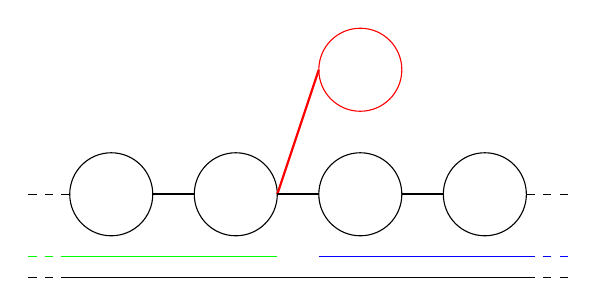
\begin{tikzpicture}[x=0.75pt,y=0.75pt,yscale=-1,xscale=1]

% begin part
\draw [dashed,black] (0, 60) -- (20, 60);
\draw (40, 60) circle (20);
\draw [fill opacity=1,thick,black] (60, 60) -- (80, 60);
\draw (100, 60) circle (20);

\draw [fill opacity=1,thick,red] (120, 60) -- (140, 0);
\draw [fill opacity=1,thick,black] (120, 60) -- (140, 60);

\draw [red] (160, 0) circle (20);

\draw (160, 60) circle (20);
\draw [fill opacity=1,thick,black] (180, 60) -- (200, 60);
\draw (220, 60) circle (20);
\draw [dashed,black] (240, 60) -- (260, 60);

\draw [dashed,green] (0, 90) -- (20,90);
\draw [green] (20, 90) -- (120, 90);

\draw [blue] (140, 90) -- (240, 90);
\draw [blue, dashed] (240, 90) -- (260,90);

\draw [dashed] (0, 100) -- (20, 100);
\draw (20, 100) -- (240, 100);
\draw [dashed] (240, 100) -- (260, 100);

\end{tikzpicture}

\end{document}

